\chapter{Experimental Evaluation}\label{chap:evaluation}

Having developed a set of transformations to normalize C and C++ programs to the theorized language subset, and having implemented an inlining optimization that takes advantage of the enabling effects of the normalization process, we devised three experiments to validate our approach:

\begin{enumerate}[label=\Alph*]
    \item Comparing a pre-existing inlining transformation's effectiveness with and without normalization, and comparing its effect to the new inlining transformation, which fully accounts for the normalization's effect.
    \item Determining the performance effects of the developed inlining optimization.
    \item Determining the enabling effects, if any, of the normalization transformations on the performance of a source-to-source automatic code parallelization tool.
\end{enumerate}

\section{Experiment A: Comparison of function inlining implementations with and without normalization}

Besides the inlining transformation that we implemented and described on Chapter \ref{chap:inlining}, the Clava standard library already possessed a previously implemented prototype of an inlining transformation, accessed through calling the \texttt{inline} method on a call node in the AST.

To compare both implementations, as well as the enabling effect of the normalization, a set of three synthetic benchmark programs were developed, featuring a variety of function calls in different contexts of the language:

\begin{itemize}
    \item A program generating 1,200,000 random two-dimensional observations and clustering them into 8 classes using a K-Means algorithm.
    \item A program multiplying two rank-35 square matrices and computing the trace of the resulting matrix.
    \item A program generating an array of 1,000,000,000 random natural numbers and performing a set of aggregations on them.
\end{itemize}

With these programs as our targets, we then proceded to run Clava to normalize and inline them as much as possible, under the following four configurations:

\begin{enumerate}
    \item Old: Using the previously implemented inlining transformation, try to inline all calls in the test programs.
    \item Normalize + Old: Normalize the test programs, then try to inline all calls with the previously implemented transformation.
    \item New: Using the newly implemented inlining transformation, try to inline all calls in the test programs.
    \item Normalize + New: Normalize the test programs, then try to inline all calls with the newly implemented transformation.
\end{enumerate}

As an evaluation metric, we chose to use the number and ratio of calls that were able to be inlined.

\begin{table}
\centering
\begin{tabular}{|c | c c c c |}
    \hline
    Scenario & \# Calls & \# No function body  & Calls Inlined & Inlining Failures \\
    \hline
    Old & 46 & 31 & 2 & 13 \\
    Normalize + Old & 50 & 31 & 6 & 13 \\
    New & 46 & 31 & 6 & 9 \\
    Normalize + New & 50 & 31 & 19 & 0 \\
    \hline
\end{tabular}
\caption{Effects of different inlining implementations with and without normalization.}
\label{tab:inlining-results}
\end{table}

Table \ref{tab:inlining-results} shows the results of the experiment. As evidenced on the first results column, we see that the normalization results on an increased number of calls being present. This is an effect of our normalization passes, namely passes to decompose expressions on the headers of iteration and selection statements, duplicating code to preserve the semantics of the normalized program. Furthermore, we see on the second column that there is a significant number of function calls that are not elegible to be inlined, owing to the body of the function not being present in the translation units that are being considered. In our case, these are calls to the C standard library, which is linked dynamically to the program.

The last two columns provide us with more interesting details.

First, we can observe the results of the program normalization. Compared with the scenarios where no normalization was made, the normalized programs are easier to inline (the old inliner goes from inlining ca. 13\% of elegible calls to inlining ca. 32\% of elegible calls, and the new inliner goes from inlining 40\% of elegible calls to inlining 100\% of elegible calls). The reason for this improvement is that, by decomposing complex expressions and by removing those expressions from the headers of control statements and other calls, we get a greater number of isolated calls and simple assignments from the value of a call to a variable, which are feasible cases for source-to-source inlining.

Secondly, we can perform a direct comparison of the two inlining implementations. From inspection of the Clava source-code, we see that to implement the inlining transformation in a less abstract language, such as Java for the case of Clava, cases where implementation can apply must be explicitly enumerated, whereas when implementing the transformation on the Javascript environment, we can rely on structural analysis and exception handling to make the transformation more general, while catching errors that pop up as exceptions. This is reflected on the comparative results of both approaches. The previously implemented inliner, which featured the exhaustive approach in Java, fails to inline calls in several occasions due to not recognizing the nodes contained within the body of the function, whereas the Javascript-based transformation need not concern itself with that filtering, leading to a ca. 27 pp. increase of successful transformations with no normalization, and, leveraging the simplification of the language afforded by the normalization process, can reach a 100\% successful inlining rate, a 68 pp. increase over the \texttt{Normalize + Old} scenario.

To validate these results, we compiled and ran the original and transformed programs, and verified that the expected output remained the same. In the case of the first scenario, additional care had to be taken to extract a useful copy of the transformed code, since one of the inlining applications produced a structuraly unsound program, therefore we saved and restored the AST before and after each inlining we tried.

There are, naturally, some factors that might affect the validity of our results:

\begin{itemize}
    \item The number and nature of the programs that we tested do not constitute an exhaustive sample of all the language constructs that a C program might contain, much less all of the constructs contained in a C++ program. There is a strong possibility that there are language features that are not accounted for and might necessitate changes and/or additions to the normalized subset or the normalization process. Nevertheless, we believe that this approach is extensible enough to bound the complexity of the resulting subset, at least for C programs and reasonably simple C++ programs used in scientific computing.
    \item The two approaches to inlining may not be strictly comparable in terms of complexity, since the older implementation takes care of some other concerns such as function body caching that the new implementation does not. However, an analysis of the implementation led us to believe that the monolithic nature of the old implementation, especially by having to deal with all the complexities of the source language, as opposed to the subset we had previously defined, played a part in its reduced flexibility.
\end{itemize}

\section{Experiment B: Performance Effects of Inlining}

To evaluate the performance effects of inlining, we took the same programs and benchmarked their runtime performance, with and without inlining, using a variety of compilers and different optimization settings. Specifically, we compiled the original and transformed programs using the GCC, clang, and CompCert toolchains, both under the \texttt{O0} (no optimizations enabled) and the \texttt{O2} (standard optimizations) optimization levels, performing, for each combination of program, compiler, presence of inlining transformation and optimization level, and measuring the average runtime duration. Inlining was performed for the entire program, by traversing the program's call graph in a depth-first fashion and inlining all calls.

We expected the following results:

\begin{itemize}
    \item Under the \texttt{O0} optimization level, we expected that, besides generally slower runtime performance, we would see a clear performance impact of the inlining transformation, varying in its sign and magnitude depending on the trade-off between the number of times a certain call is performed, and the code bloat resulting from the duplicated function bodies. Specifically, we theorized that inlining small functions that are called often would result in performance gains, and that inlining bigger functions with less frequent calls would have smaller gains or even negative performance effects.
    \item Under the \texttt{O2} optimization level, we expected that there would be little performance effect, as the compilers under test already should perform several code optimization transformations, including inlining, and so the source-code level transformation would have less of an effect.
\end{itemize}

\begin{figure}
    \centering
    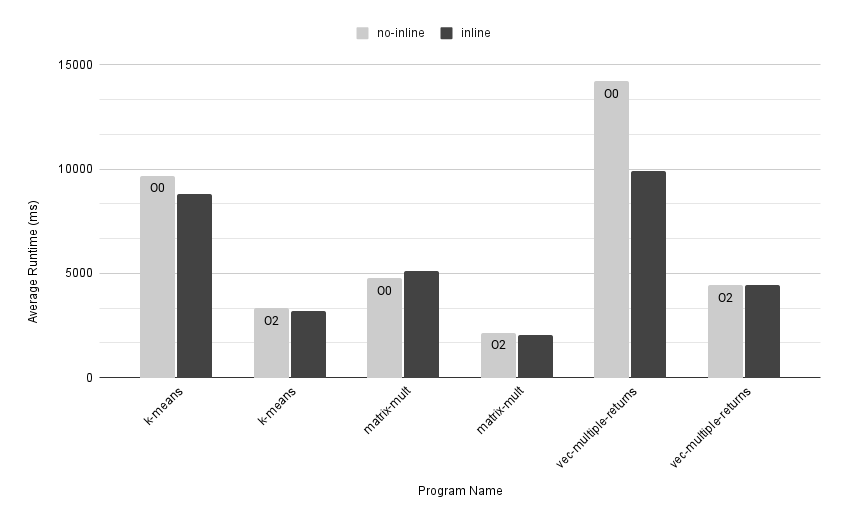
\includegraphics[width=\textwidth]{figures/benchmark-chart.png}
    \caption{Microbenchmark performance, inlining vs no inlining. Segmented by program, optimization level.}
    \label{fig:expb-chart}
\end{figure}

Figure \ref{fig:expb-chart} shows a high-level visualization of the results of this experiment. For each program, two sets of columns show the average runtime in several configurations. One set presents the results with no compiler optimizations (\texttt{O0}) and the other presents the results with optimizations enabled (\texttt{O2}). The columns in light grey show the average runtime of the original program for that configuration, and the columns in dark grey show the average runtime of the program after the source-level inlining was applied.

In aggregate, the results obtained fell within the expectations we had set before. The \texttt{k-means} and \texttt{matrix-mult} programs, that featured larger functions and less iterations comparatively to the number of calls, had less expressive and mixed performance impacts on the runtime performance of the program when transformed. Specifically, on the \texttt{O0} configuration, K-Means compute performance was ca. 9\% faster, but Matrix Multiplication was ca. 7\% slower. On the other had, the \texttt{vec-multiple-returns} program, which featured a tight-loop more easily dominated by a call to a small function, experienced a ca. 30\% reduction in average runtime. Under the \texttt{O2} configuration, the performance effects were generally less expressive, as expected, but, surprisingly, we saw an inversion on the magnitudes of the performance effects when comparing k-means and matrix multiplication with the array slice aggregation program. While the performance effect on \texttt{vec-multiple-returns} dropped to ca. -0.34\%, source-level inlining decreased the average runtime of \texttt{k-means} and \texttt{matrix-mult} by ca. 4.5\% and 5.2\%, respectively. A possible explanation is that the underlying compilers might not have inlined certain calls, without the source-level inlining, and the inlined function would enable more optimizations to be performed at the global analysis level.

\begin{table}[]
\centering
\begin{tabular}{|c|c|c|ccc|}
\hline
\multirow{2}{*}{Compiler} & \multirow{2}{*}{Opt. Level} & \multirow{2}{*}{Inlining} & \multicolumn{3}{c|}{Program} \\
\cline{4-6} 
 & & & vec-multiple-returns & matrix-mult & k-means \\
\hline
\multirow{4}{*}{CompCert} & \multirow{2}{*}{O0} & Yes & 4462.37 & 2864.06 & 3392.99 \\
 & & No & 4454.64 & 2792.85 & 4630.94 \\
 & \multirow{2}{*}{O2} & Yes & 4443.17 & 2694.85 & 4379.61 \\
 & & No & 4445.98 & 2796.52 & 4830.31 \\
\hline
\multirow{4}{*}{Clang} & \multirow{2}{*}{O0} & Yes & 6723.64 & 6376.61 & 11379.62 \\
 & & No & 19771.91 & 5714.09 & 11717.30 \\
 & \multirow{2}{*}{O2} & Yes & 4418.02 & 1619.00 & 1972.17 \\
 & & No & 4420.98 & 1889.16 & 1978.27 \\
\hline
\multirow{4}{*}{GCC} & \multirow{2}{*}{O0} & Yes & 18486.90 & 6059.89 & 11662.09 \\
 & & No & 18456.40 & 5784.92 & 12703.43 \\
 & \multirow{2}{*}{O2} & Yes & 4451.80 & 1840.78 & 3182.59 \\
 & & No & 4401.42 & 1806.91 & 3173.13 \\
\hline
\end{tabular}
\caption{Runtime performance (ms) for each program, segmented by compiler, optimization level, source-level inlining.}
\label{tab:expb-pivot}
\end{table}

Zooming in from the aggregate results to the results separated by compiler, we come upon other interesting results. Table \ref{tab:expb-pivot} shows the runtime performance numbers, segmented by compiler, optimization level, and whether source-level inlining was applied. There, we can see that the results actually follow two modes regarding the behavior presented by different compilers. Clang and GCC, which are older but have had more optimization work put it, present a stark difference between the code that is generated with and without optimization. On the other hand, CompCert seems to generate comparatively faster code without optimizing, but does not present large gains in performance when code optimization is enabled. Comparing both sets, we see that the optimized code from GCC and Clang seems to be faster than optimized code from CompCert. Nevertheless, source-level inlining seems to be worthwhile in general, especially when considering that the transformations that we developed were prototypical and limited in nature, so further work may result in even greater performance effects. In some cases, there is a sizable performance benefit of applying it, such as on array slice aggregation with O0 and Clang, and on k-means with CompCert, in which it performs faster than even the optimized code, supporting our hypothesis that source-to-source transformation work will be especially impactful on less developed compilers.

To validate our results, we measured, for each configuration, 8 runs of the benchmark. Besides recording the average runtime duration, we recorded the standard deviation of our observations. For \texttt{vec-multiple-returns} and \texttt{k-means}, the average standard deviation of our observations was well under 1\% of the measured average runtime duration. For \texttt{matrix-mult}, the measurement standard deviations were somewhat higher, but still within 10\% of the magnitude of the observations in all cases.

Of course, some factors do limit our analysis and confidence in these results:

\begin{itemize}
    \item The programs that we tested only represent a subset of the types of computation performed in C and C++, and thus the results might not be representative of the effect of the transformation on the overall corpus of existing C and C++ code. A larger set of codes might be tested to further validate the results.
    \item Only one hardware target was used in the test and, by extension, only one set of platforms and computation models. As an extension, it might prove useful to test this optimization on different platforms, different hardware targets (featuring different single-clock speeds, cache sizes, etc.) and different computation models (GPU, FPGAs with HLS, etc.).
    \item We only developed and tested one optimizing transformation. Other transformations might be more or less worthwhile to be executed at different levels of abstraction, and so we may not draw overly general conclusions about the potential use of the source-to-source compilation approach to optimization.
\end{itemize}

Nevertheless, we can conclude that there are some measurable effects of performing inlining on the source-code level on the performance of certain C and C++ programs, under different compilers.

\section{Experiment C: Enabling Effects of Normalization on Automatic Parallelizer}

The last experiment we performed was running a well-known benchmark through an existing source to source optimization tool to validate the effect of our normalization code. To do so, we selected the following benchmark and tool:

\begin{itemize}
    \item As the benchmark, we selected the NAS Parallel Benchmarks. These benchmarks, originally produced by NASA, aim to test the performance of parallel computing systems, which paired well with the tool we chose. Furthermore, an implementation of these benchmarks was already packaged in a compatible way with the LARA Framework's benchmark facility.
    \item As the tool to test, we chose Autopar-Clava\cite{Arabnejad2018}, an automatic parallelization transformation for Clava. This tool  analyses a program's loops, its inductive variables, and its memory access patterns \cite{Arabnejad2020} to insert OpenMP directives in the code, yielding a parallelized version of it. We chose it for our evaluation due to its presence in the Clava standard library, as well as previous expertise in the lab developing and using it. Furthermore, Autopar-Clava was described by its authors as using Clava's built-in inlining facility, so we hoped to be able to compare this implementation to our own newly-implemented inlining facility.
\end{itemize}

We aimed this experiment to explore the enabling effects of the newly developed normalization and inlining transformations on the effect of further optimizations. Thus, from the NAS benchmark suite, we picked a variety of tests, in several classes of magnitude. We chose the tests in a way that ensured a variety of source-code constructs was represented, and chose the magnitudes that would be big enough to ensure confidence in the results, yet not too large, in the interest of time. Specifically, we picked benchmarks for a Block Tri-diagonal matrix equation solver (BT), a Conjugate Gradient computation kernel for linear differential equation solving (GG), a discrete 3D fast Fourier Transform computation kernel (FT), a Lower-Upper matrix solver using the Gauss-Seidel method (LU), a differential equation solver kernel using the Multi-grid method (MG), and a Scalar pentadiagonal matrix solver (SP), using the magnitude classes W, A, and B, which range in runtime duration from ca. 0.5 seconds to ca. 8 minutes.

Afterwards, we laid out four scenarios:

\begin{enumerate}
    \item Baseline: benchmark the selected benchmark instances, without modification.
    \item Autopar: parallelize the selected benchmark instances using Autopar-Clava, with no preceding transformations, and benchmark the transformed programs.
    \item Normalize: normalize the selected benchmark instances to our predefined language subset, parallelize them, and benchmark the tranformed programs.
    \item Inline: modify Autopar-Clava to disable the built-in inlining transformation; normalize the selected benchmark instances to our predefined language subset, perform automated inlining with our newly developed inlining transformation, parallelize them, and benchmark the transformed programs (this scenario remained untested).
\end{enumerate}

As an evaluation metric, we again chose the runtime duration of the benchmarks, seeking to minimize it. Our expectation was that Autopar-processed code would perform better than the baseline on our multi-core workstation, with the exception of the FT benchmark, which was expected to slow down, as per the results previously obtained in \cite{Arabnejad2020}.

% Please add the following required packages to your document preamble:
% \usepackage{multirow}
\begin{table}[]
\centering
\begin{tabular}{|c|c|ccc|}
\hline
\multirow{2}{*}{Program} & \multirow{2}{*}{\begin{tabular}[c]{@{}c@{}}Magnitude\\ Class\end{tabular}} & \multicolumn{3}{c|}{Scenario}    \\ \cline{3-5} 
                         &                                                                            & Baseline & Autopar   & Normalize \\ \hline
\multirow{3}{*}{BT}      & W                                                                          & 5.32     & 22.87     & 5.41      \\
                         & A                                                                          & 113.46   & 59,979.11 & 118.31    \\
                         & B                                                                          & 468.25   & -         & 517.56    \\ \hline
\multirow{3}{*}{CG}      & W                                                                          & 0.57     & 0.05      & 0.59      \\
                         & A                                                                          & 2.00     & 0.11      & 2.04      \\
                         & B                                                                          & 90.21    & 7.07      & 95.97     \\ \hline
\multirow{3}{*}{FT}      & W                                                                          & 0.44     & 11.93     & 0.46      \\
                         & A                                                                          & 7.93     & 253.65    & 8.13      \\
                         & B                                                                          & 95.16    & 5,771.09  & 98.83     \\ \hline
\multirow{3}{*}{LU}      & W                                                                          & 16.46    & 61.10     & 18.31     \\
                         & A                                                                          & 112.25   & 947.73    & 116.44    \\
                         & B                                                                          & 467.46   & 6,247.38  & 481.04    \\ \hline
\multirow{3}{*}{MG}      & W                                                                          & 0.58     & 0.08      & 0.64      \\
                         & A                                                                          & 4.62     & 0.60      & 5.04      \\
                         & B                                                                          & 20.98    & 1.85      & 22.94     \\ \hline
\multirow{3}{*}{SP}      & W                                                                          & 18.40    & 23.71     & 19.43     \\
                         & A                                                                          & 104.44   & 164.17    & 110.02    \\
                         & B                                                                          & 437.79   & 706.49    & 458.73    \\ \hline
\end{tabular}
\caption{Runtime duration of benchmarks (s), segmented by scenario, program, magnitude class.}
\label{tab:expc-results}
\end{table}

Table \ref{tab:expc-results} shows the resulting runtime duration for each of our scenarios. Compared to the baseline, the Autopar scenario showed definite effects on the runtime performance of different benchmarks. In the case of the CG and MG program, we were able to obtain concrete speedups, on the order of 7.25x to 18.18x. FT also performed as seen in \cite{Arabnejad2020}, being several tens of times slower than the baseline result. However, we could not reproduce the results previously seen for the BT, LU and SP cases. In the case of LU, slight slowdowns occured. In the case of LU and BT, though, the performance degradation seemed to scale with the benchmark magnitude super-linearly, leading to not being able to obtain any results for BT at magnitude class B. We suspected that the two-chiplet design of our workstation's CPU could be to blame for the slowdown, owing to slower communication between cores, but we were also unable to reproduce these results using codes from the original publication and on another workstation, which did not share the same hardware peculiarities. Another hypothesis for the slowdown was that the loops that were parallelized did not perform enough work on their own, so the overhead of parallelizing them resulted in performance degradation.

Compared to the previous two scenarios, the Normalize scenario evidenced a surprising result. Autopar-Clava was not able to parallelize any loops, and thus the runtime performance was roughly similar to the baseline scenario, as opposed to being similar to the Autopar scenario. Analyzing the output logs, we realized that Autopar relied on analyzing \texttt{for} statements to identify possible parallelization opportunities. Since our normalization transformation removed \texttt{for} statements from the language subset, the parallelizer was not able to perform its job. In the absence of more time for reworking the normalization transformations to account for this use, we carried out with analyzing the results of this experiment and drawing conclusions, having cancelled testing for scenario Inline, since the same lack of results was certain.

This experiment showed us that there is still room for reconsideration of the subset that we defined. For statements are an important expressive construct for use in writing a program but, guided by the fact that compilers are able to identify loop structures, their invariants and induction variables, we considered on a theoretical sense that they would not be necessary on our language subset. However, even if not strictly necessary, the construct is used for automated tools and analyses in a source-to-source context, and thus removing it may not be the best decision. To reintroduce the construct into the subset, we might consider the following two routes:

\begin{itemize}
    \item Only transforming for loops into while loops conditionally, based on the characteristics of the statements in the header. For example, we could keep simple loops, such as a canonical loop comparing against a constant or variable, while processing loops that compare against the return value of a call. \textit{In extremis}, we could rely on user input of some sort to mark instances to be kept.
    \item We can keep our transformation to a while loop, and then follow it with passes for loop canonicalization, such as loop invariant code motion, induction variable analysis and so on, reconstituting a normalized version of the for loop afterwards. This approach is certainly more complex, but might work better in the general case.
\end{itemize}

\section{Summary}

In this chapter, we presented three experiments to try and understand how source-code normalization affects the possibility and ease of implementing program optimizations on the source-code level. The first experiment showed that after normalizing the code, two independent implementations of a function inlining transformation were able to inline calls in more situations that they were able to before. The second experiment validated our case study in implementing a performance optimization in a source-to-source context, since performance effects of the transformation were evident, especially on less optimizing compiler choices and configurations. The third experiment had negative results. Besides having had trouble reproducing a baseline that was in line with previous works on the tool we chose, our normalization process removed primitives on which the tool relied and greatly diminished its effect. While not invalidating our approach, it gave us a perspective on how our work can be improved upon.
